\documentclass[12pt, a4paper]{article}

% --- ESSENTIAL PACKAGES ---
\usepackage[utf8]{inputenc}
\usepackage[english]{babel}
\usepackage[T1]{fontenc}
\usepackage{graphicx}         % To insert images (e.g., ANSYS screenshots)
\usepackage{amsmath, amsfonts} % For mathematical equations
\usepackage{geometry}         % Page margins configuration
\geometry{top=2.5cm, bottom=2.5cm, left=2.5cm, right=2.5cm}
\usepackage{float}            % To force figure placement [H]
\usepackage{booktabs}         % For high-quality tables
\usepackage{xcolor}           % For text/code colors
\usepackage[hidelinks]{hyperref} % For hyperlinks and interactive table of contents
\usepackage{subcaption}
\graphicspath{{Images/}}      % Calling the Images folder

% --- HEADER AND FOOTER ---
\usepackage{fancyhdr}
\pagestyle{fancy}
\fancyhf{}
\rhead{ANSYS CFD Simulation Project}
\lhead{Aerodynamic Analysis}
\rfoot{Page \thepage}

% --- DOCUMENT INFORMATION ---
\title{\textbf{ANSYS CFD Simulation} \\ 
	\large Aerodynamic Analysis and Airflow Around a Vehicle}
\author{\textbf{Written by:} Friedly WOLI}
\date{\today}

% --- BEGIN DOCUMENT ---
\begin{document}
	
	\maketitle
	\thispagestyle{fancy}
	
	\section{Introduction and Theoretical Framework}
	
	To describe the mechanical response of a continuous medium (material body), we require constitutive assumptions. The primary problem in continuum mechanics is to determine:
	\begin{itemize}
		\item The deformed configuration $\omega$ and the vector field of displacement $\mathbf{u} = \mathbf{u}(p)$.
		\item The infinitesimal strain tensor field and the stress tensor field.
	\end{itemize}
	In total, the unknowns of the problem consist of 15 scalar fields. 
	
	At our disposal, we have 9 fundamental equations:
	\begin{itemize}
		\item 6 kinematic relations (strain-displacement relations).
		\item 3 equilibrium equations (balance of linear momentum).
	\end{itemize}
	
	Consequently, there is a deficit of 6 equations missing from the general system—namely, the specific behavior of the material. These relations define the constitutive class $\mathcal{C}$ of the body $\omega$, representing the set of all dynamically admissible processes for $\omega$.
	
	\section{Restrictions on Constitutive Equations}
	
	The most general link between the Cauchy stress tensor $\boldsymbol{\sigma}$ and the motion can be expressed as:
	\begin{equation}
		\sigma_{ij} = \sigma_{ij}(\mathbf{u}, \boldsymbol{\epsilon}, \boldsymbol{\omega}, \dots)
	\end{equation}
	
	General physical requirements must be fulfilled by any valid constitutive equation:
	\begin{itemize}
		\item The mechanical behavior of the body must be independent of absolute position and orientation.
		\item Any dependence upon rigid-body translations and rotations must vanish, reducing the dependency to:
		\begin{equation}
			\boldsymbol{\sigma} = \boldsymbol{\sigma}(\boldsymbol{\epsilon}, \dots)
		\end{equation}
	\end{itemize}
	
	Materials whose constitutive equations depend upon the strain rate and strain (such as viscous fluids, including Newtonian fluids) follow constitutive relations of the form:
	\begin{equation}
		\sigma_{ij} = -p\mathbf{I} + 2\mu\boldsymbol{\epsilon} + \lambda \text{tr}(\boldsymbol{\epsilon})\mathbf{I}
	\end{equation}
	where $p$ represents the thermodynamic pressure, and $\mu$ and $\lambda$ are the coefficients of dynamic and bulk viscosity, respectively.
	
	\section{Fluid Assumptions and Governing Equations}
	
	Air is modeled as a continuous fluid. For standard aerodynamic analyses at moderate speeds, it can be approximated as incompressible, meaning that each dynamical process is isochoric (volume-preserving) for all time $t$.
	
	An ideal fluid body $\omega$ has a constitutive class $\mathcal{C}$ defined by isochoric Eulerian dynamical processes where density $\rho$ remains constant ($\rho = \rho_0 = \text{constant}$). This implies that air behaves as an incompressible, homogeneous fluid in which the stress is primarily characterized by pressure in every flow regime.
	
	For such fluids, the governing momentum conservation equations simplify to:
	\begin{align}
		\nabla \cdot \boldsymbol{\sigma} + \mathbf{b} &= \rho_0 \frac{\partial \mathbf{v}}{\partial t} \\
		-\nabla p + \mathbf{b} &= \rho_0 \mathbf{a} \\
		\nabla \cdot \mathbf{v} &= 0
	\end{align}
	where $\mathbf{v}$ is the velocity vector field and $\mathbf{b}$ represents body forces.
	
	\section{CFD Simulation Steps}
	
	\subsection{Geometry and Symmetry}
	The computational geometry was imported from a CAD model representing the vehicle. To optimize computational cost and resource usage, the simulation takes advantage of physical symmetry, modeling only half of the vehicle along the longitudinal symmetry plane.
	
	\begin{figure}[H]
		\centering
		% Replace 'cad_geometry.png' with your actual image file name in the Images/ folder
		\framebox{\parbox{0.8\textwidth}{\centering \vspace{2cm} [Insert CAD Geometry Image: \texttt{cad\_geometry.png}] \vspace{2cm}}}
		\caption{Vehicle CAD Geometry and Computational Domain (Symmetry Model)}
		\label{fig:cad_geometry}
	\end{figure}
	
	\subsection{Boundary Conditions}
	Named selections were applied to define the domain boundaries:
	\begin{itemize}
		\item \textbf{Inlet:} Velocity inlet set to $20\,\text{m/s}$ (representing an average cruising speed for a car).
		\item \textbf{Outlet:} Pressure outlet condition applied.
		\item \textbf{Walls:} No-slip boundary conditions assigned to the vehicle surface and ground.
		\item \textbf{Symmetry:} Symmetry plane defined along the vehicle centerline.
	\end{itemize}
	
	\subsection{Meshing}
	An unstructured mesh was generated with local refinements near the vehicle surface to capture high-gradient boundary layer effects, transitioning to larger mesh elements in the far-field domain. Spatial discretization utilized a second-order upwind scheme for enhanced accuracy.
	
	\begin{figure}[H]
		\centering
		% Replace 'mesh_domain.png' with your actual image file name in the Images/ folder
		\framebox{\parbox{0.8\textwidth}{\centering \vspace{2cm} [Insert Mesh Screenshot: \texttt{mesh\_domain.png}] \vspace{2cm}}}
		\caption{Computational Mesh Setup Showing Local Refinement around the Vehicle}
		\label{fig:mesh_domain}
	\end{figure}
	
	\subsection{Results and Discussion}
	
	\subsubsection{Velocity Contours}
	The velocity contour plot illustrates the local speed variations across the flow field. A distinct stagnation point is observed at the front of the vehicle where the incoming airflow decelerates to zero velocity.
	
	\begin{figure}[H]
		\centering
		% Replace 'velocity_contour.png' with your actual image file name in the Images/ folder
		\framebox{\parbox{0.8\textwidth}{\centering \vspace{2cm} [Insert Velocity Contour Screenshot: \texttt{velocity\_contour.png}] \vspace{2cm}}}
		\caption{Velocity Contour Plot Showing Flow Stagnation and Local Speed Variations}
		\label{fig:velocity_contour}
	\end{figure}
	
	\subsubsection{Velocity Vectors}
	The velocity vector plots depict the airflow impinging on the vehicle's front fascia, followed by smooth boundary layer development and subsequent flow separation over the windshield and roofline.
	
	\begin{figure}[H]
		\centering
		% Replace 'velocity_vectors.png' with your actual image file name in the Images/ folder
		\framebox{\parbox{0.8\textwidth}{\centering \vspace{2cm} [Insert Velocity Vectors Screenshot: \texttt{velocity\_vectors.png}] \vspace{2cm}}}
		\caption{Velocity Vector Field Across the Vehicle Symmetry Plane}
		\label{fig:velocity_vectors}
	\end{figure}
	
	\subsubsection{Streamlines and Wake Region}
	Streamline visualizations highlight the aerodynamic wake formed behind the vehicle, showing recirculation zones and turbulent mixing downstream in the rear detachment region.
	
	\begin{figure}[H]
		\centering
		% Replace 'streamlines_wake.png' with your actual image file name in the Images/ folder
		\framebox{\parbox{0.8\textwidth}{\centering \vspace{2cm} [Insert Streamlines Screenshot: \texttt{streamlines\_wake.png}] \vspace{2cm}}}
		\caption{3D Velocity Streamlines Demonstrating Downstream Wake Recirculation}
		\label{fig:streamlines}
	\end{figure}
	
	
	\subsection{Comment}
	
	
	
	
	
	\section{General picture }
	
	\subsection{geometry}
	\begin{figure}[htbp]
		\centering
		% Top Left Image
		\begin{subfigure}[b]{0.48\textwidth}
			\centering
			% Replace 'cad_geometry.png' with your actual file name
			%\includegraphics[width=\textwidth]{cad_geometry.png} 
			\caption{Imported CAD geometry}
			\label{fig:cad_geom}
		\end{subfigure}
		\hfill % Adds horizontal space between the figures
		% Top Right Image
		\begin{subfigure}[b]{0.48\textwidth}
			\centering
			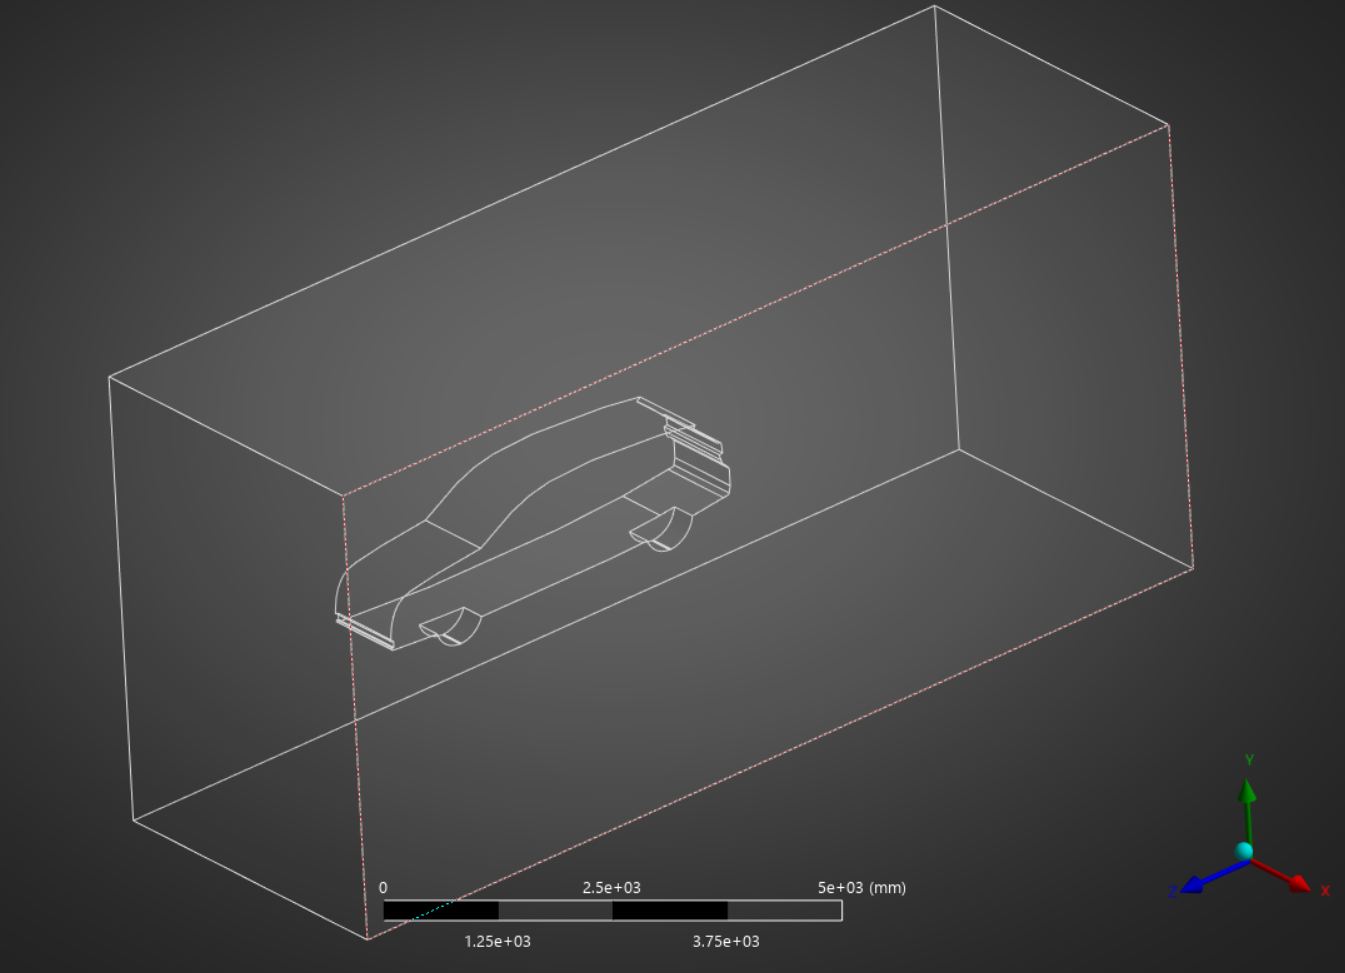
\includegraphics[width=\textwidth]{geometry1.png}
			\caption{Control volume and vehicle geometry}
			\label{fig:mesh}
		\end{subfigure}
		
		\vspace{0.5cm} % Adds vertical space between the rows
		
		% Bottom Left Image
		\begin{subfigure}[b]{0.48\textwidth}
			\centering
			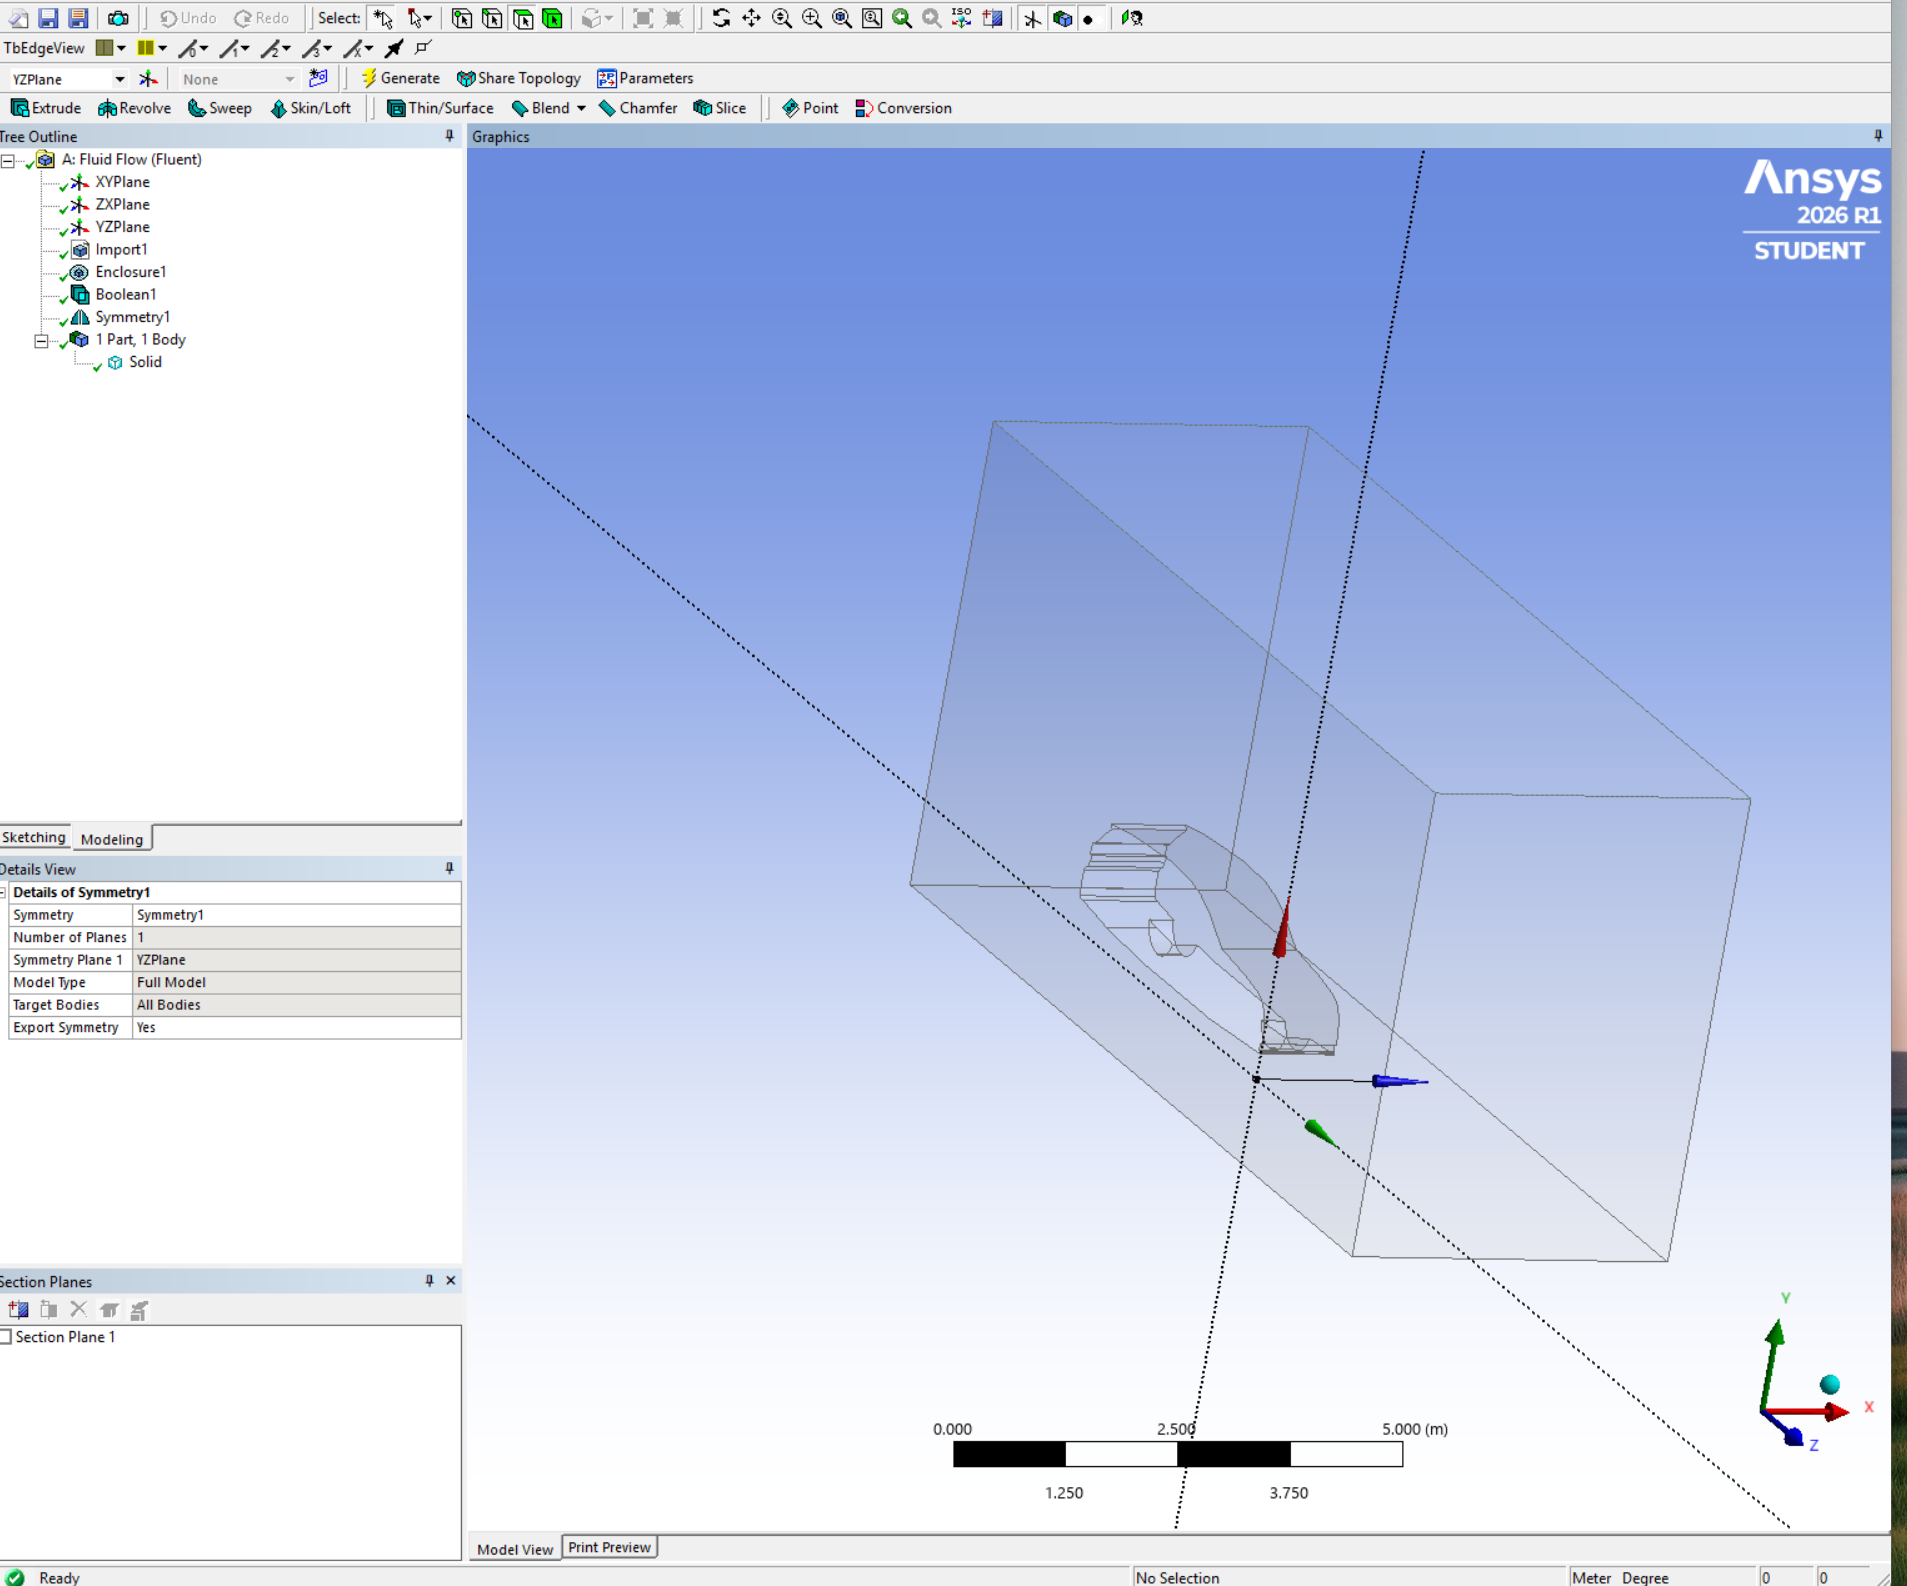
\includegraphics[width=\textwidth]{symetry_for simulation.png}
			\caption{Plane of symmetry}
			\label{fig:contour}
		\end{subfigure}
		\hfill
		% Bottom Right Image
		\begin{subfigure}[b]{0.48\textwidth}
			\centering
			%\includegraphics[width=\textwidth]{streamlines_wake.png}
			\caption{Streamlines and wake region}
			\label{fig:wake}
		\end{subfigure}
		
		\caption{ANSYS CFD simulation results for the vehicle aerodynamics analysis.}
		\label{fig:all_results}
	\end{figure}
	
	
	\subsection{meshing}
	
	\begin{figure}[htbp]
		\centering
		% Top Left Image
		\begin{subfigure}[b]{0.48\textwidth}
			\centering
			% Replace 'cad_geometry.png' with your actual file name
			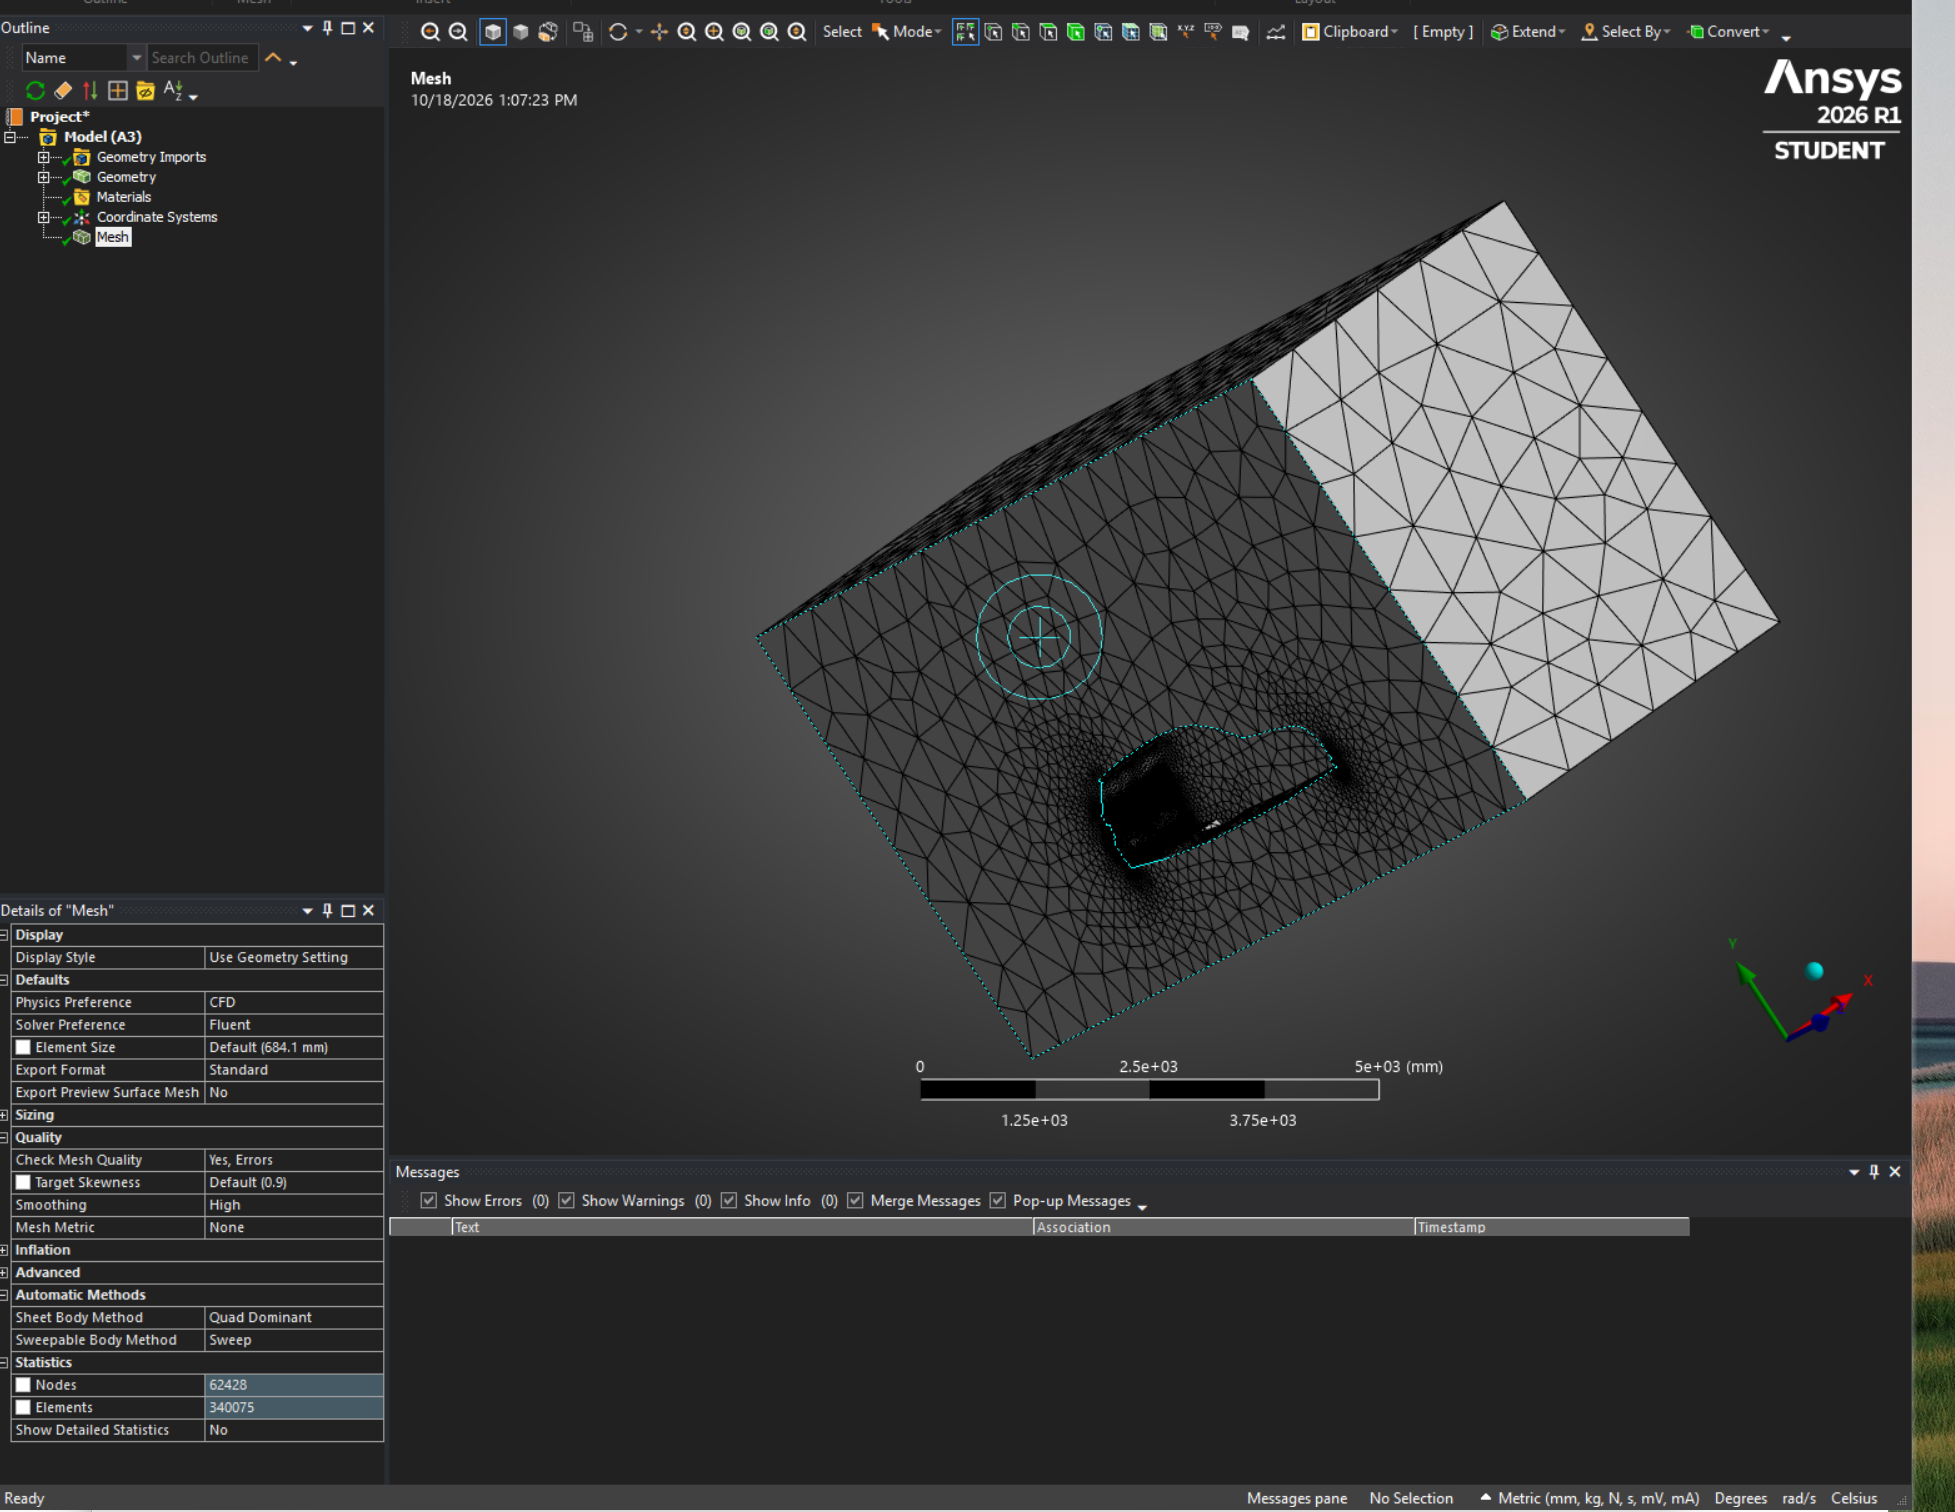
\includegraphics[width=\textwidth]{meshing_generate_1.png} 
			\caption{Imported CAD geometry}
			\label{fig:cad_geom}
		\end{subfigure}
		\hfill % Adds horizontal space between the figures
		% Top Right Image
		\begin{subfigure}[b]{0.48\textwidth}
			\centering
			%\includegraphics[width=\textwidth]{mesh_domain.png}
			\caption{Mesh refinement around vehicle}
			\label{fig:mesh}
		\end{subfigure}
		
		\vspace{0.5cm} % Adds vertical space between the rows
		
		% Bottom Left Image
		\begin{subfigure}[b]{0.48\textwidth}
			\centering
			%\includegraphics[width=\textwidth]{velocity_contour.png}
			\caption{Velocity contours and stagnation point}
			\label{fig:contour}
		\end{subfigure}
		\hfill
		% Bottom Right Image
		\begin{subfigure}[b]{0.48\textwidth}
			\centering
			%\includegraphics[width=\textwidth]{streamlines_wake.png}
			\caption{Streamlines and wake region}
			\label{fig:wake}
		\end{subfigure}
		
		\caption{ANSYS CFD simulation results for the vehicle aerodynamics analysis.}
		\label{fig:all_results}
	\end{figure}
		
	\subsection{boundaries condition}
	

	\begin{figure}[htbp]
		\centering
		% Top Left Image
		\begin{subfigure}[b]{0.48\textwidth}
			\centering
			% Replace 'cad_geometry.png' with your actual file name
			%\includegraphics[width=\textwidth]{cad_geometry.png} 
			\caption{Imported CAD geometry}
			\label{fig:cad_geom}
		\end{subfigure}
		\hfill % Adds horizontal space between the figures
		% Top Right Image
		\begin{subfigure}[b]{0.48\textwidth}
			\centering
			%\includegraphics[width=\textwidth]{mesh_domain.png}
			\caption{Mesh refinement around vehicle}
			\label{fig:mesh}
		\end{subfigure}
		
		\vspace{0.5cm} % Adds vertical space between the rows
		
		% Bottom Left Image
		\begin{subfigure}[b]{0.48\textwidth}
			\centering
			%\includegraphics[width=\textwidth]{velocity_contour.png}
			\caption{Velocity contours and stagnation point}
			\label{fig:contour}
		\end{subfigure}
		\hfill
		% Bottom Right Image
		\begin{subfigure}[b]{0.48\textwidth}
			\centering
			%\includegraphics[width=\textwidth]{streamlines_wake.png}
			\caption{Streamlines and wake region}
			\label{fig:wake}
		\end{subfigure}
		
		\caption{ANSYS CFD simulation results for the vehicle aerodynamics analysis.}
		\label{fig:all_results}
	\end{figure}
			
		\subsection{results}
		
		\begin{figure}[htbp]
			\centering
			% Top Left Image
			\begin{subfigure}[b]{0.48\textwidth}
				\centering
				% Replace 'cad_geometry.png' with your actual file name
				%\includegraphics[width=\textwidth]{cad_geometry.png} 
				\caption{Imported CAD geometry}
				\label{fig:cad_geom}
			\end{subfigure}
			\hfill % Adds horizontal space between the figures
			% Top Right Image
			\begin{subfigure}[b]{0.48\textwidth}
				\centering
				%\includegraphics[width=\textwidth]{mesh_domain.png}
				\caption{Mesh refinement around vehicle}
				\label{fig:mesh}
			\end{subfigure}
			
			\vspace{0.5cm} % Adds vertical space between the rows
			
			% Bottom Left Image
			\begin{subfigure}[b]{0.48\textwidth}
				\centering
				%\includegraphics[width=\textwidth]{velocity_contour.png}
				\caption{Velocity contours and stagnation point}
				\label{fig:contour}
			\end{subfigure}
			\hfill
			% Bottom Right Image
			\begin{subfigure}[b]{0.48\textwidth}
				\centering
				%\includegraphics[width=\textwidth]{streamlines_wake.png}
				\caption{Streamlines and wake region}
				\label{fig:wake}
			\end{subfigure}
			
			\caption{ANSYS CFD simulation results for the vehicle aerodynamics analysis.}
			\label{fig:all_results}
		\end{figure}
				

	
	
	
\end{document}